\documentclass[11pt]{article}
%% Packages for bibliography
% Use either natbib or biblatex
%\usepackage[round]{natbib}  

\usepackage[backend=biber,
            bibstyle=authoryear,
            citestyle=authoryear,
            maxbibnames=9,
            maxcitenames=2,
            dashed=false,
            firstinits=true,]
            {biblatex}
 
\usepackage{bibentry}

% See other styles in sharelatex
% https://www.sharelatex.com/learn/Biblatex_bibliography_styles


%% Hyperref authoryear style
% https://tex.stackexchange.com/questions/1687/hyperlink-name-with-biblatex-authoryear
\DeclareCiteCommand{\cite}
  {\usebibmacro{prenote}}
  {\usebibmacro{citeindex}%
   \printtext[bibhyperref]{\usebibmacro{cite}}}
  {\multicitedelim}
  {\usebibmacro{postnote}}

\DeclareCiteCommand*{\cite}
  {\usebibmacro{prenote}}
  {\usebibmacro{citeindex}%
   \printtext[bibhyperref]{\usebibmacro{citeyear}}}
  {\multicitedelim}
  {\usebibmacro{postnote}}

\DeclareCiteCommand{\parencite}[\mkbibparens]
  {\usebibmacro{prenote}}
  {\usebibmacro{citeindex}%
    \printtext[bibhyperref]{\usebibmacro{cite}}}
  {\multicitedelim}
  {\usebibmacro{postnote}}

\DeclareCiteCommand*{\parencite}[\mkbibparens]
  {\usebibmacro{prenote}}
  {\usebibmacro{citeindex}%
    \printtext[bibhyperref]{\usebibmacro{citeyear}}}
  {\multicitedelim}
  {\usebibmacro{postnote}}

\DeclareCiteCommand{\footcite}[\mkbibfootnote]
  {\usebibmacro{prenote}}
  {\usebibmacro{citeindex}%
  \printtext[bibhyperref]{ \usebibmacro{cite}}}
  {\multicitedelim}
  {\usebibmacro{postnote}}

\DeclareCiteCommand{\footcitetext}[\mkbibfootnotetext]
  {\usebibmacro{prenote}}
  {\usebibmacro{citeindex}%
   \printtext[bibhyperref]{\usebibmacro{cite}}}
  {\multicitedelim}
  {\usebibmacro{postnote}}

\DeclareCiteCommand{\textcite}
  {\boolfalse{cbx:parens}}
  {\usebibmacro{citeindex}%
   \printtext[bibhyperref]{\usebibmacro{textcite}}}
  {\ifbool{cbx:parens}
     {\bibcloseparen\global\boolfalse{cbx:parens}}
     {}%
   \multicitedelim}
  {\usebibmacro{textcite:postnote}}
  
  
  
  
%% Packages for figures
\usepackage{graphicx}			%% Path to figures and more I guess
\usepackage{epstopdf}			%% Needed for .eps files
\usepackage{subfig}		    	%% Array of figures (incompatible with subcaption)
\usepackage{float} 				%% Force floats position


%% Packages for tables
\usepackage{tabularx}			%% Advanced tables
\usepackage{booktabs}			%% http://www.tablesgenerator.com/
\usepackage{multirow}			%% Combine cells of tables
\usepackage[flushleft]{threeparttable} % Add notes to a table
\usepackage{adjustbox} 			%% Give maximum height-width
\usepackage{rotating}			%% Sideways table
%\usepackage{floatrow}			%% Table and figure side by side


%% Packages for captions
\usepackage[				    	%% Caption style
font=small,labelfont=bf]
{caption}
%\usepackage{subcaption}			%% Make captions for subfigures
\captionsetup{parskip=5pt}	    	%% Set the caption paragraph spacing


%% Packages for math
\usepackage{amssymb}
\usepackage{mathrsfs}
\usepackage{amsthm}
\usepackage[fleqn]{amsmath}		%% Subequations and more I guess
\usepackage{nicefrac}			%% Cool fractions
\usepackage[fleqn]{cases}		%% Piecewise function
\usepackage{bm}					%% Bold greek symbols in math mode
\usepackage{dsfont}             %% Caligraphic math months
\usepackage{commath}            %% \norm


%% Packages for links
\usepackage{color}				%% Color for the text
\usepackage{xcolor}				%% Advanced color for the text
\usepackage[					%% Clickable links
hypertexnames=false,
bookmarksopen=true]{hyperref}	
\hypersetup{
    colorlinks,
    linkcolor={blue!00!black},
    citecolor={blue!30!black},
    urlcolor={blue!30!black}}
\usepackage{url}				%% Hyperlinks to webs
% The option hypertexnames=false is set to prevent problems when the chapter numbering is modified (appendices)


%% Dots for the table of contents
\usepackage{tocloft}
\renewcommand{\cftpartleader}{\cftdotfill{\cftdotsep}} % for parts
\renewcommand{\cftchapleader}{\cftdotfill{\cftdotsep}} % for chapters
\renewcommand{\cftsecleader}{\cftdotfill{\cftdotsep}} % for sections, if you really want! (It is default in report and book class (So you may not need it).
% https://tex.stackexchange.com/questions/53898/how-to-get-lines-with-dots-in-the-table-of-contents-for-sections
% ----------------------------------------------------------------


%% Package for nomenclature
\usepackage[intoc]{nomencl}
\makenomenclature
% Create nomenclature groups
\usepackage{etoolbox}
\renewcommand\nomgroup[1]{%
  \item[\large\bfseries
  \ifstrequal{#1}{A}{Symbols}{%
  \ifstrequal{#1}{B}{Greek Letters}{%
  \ifstrequal{#1}{C}{Acronyms}{%
  \ifstrequal{#1}{D}{Subscripts}{}}}}%
]\vspace{12pt}}
% Add the units to nomenclature
\newcommand{\nomunit}[1]{%
\renewcommand{\nomentryend}{\hspace*{\fill}#1}}
% The difficult thing is to prepare the compilation order
% Check the documentation in the future


%% Package for glossary
\usepackage[toc,nonumberlist]{glossaries}
%\setglossarystyle{long}
\setglossarystyle{altlist}
\renewcommand{\glsnamefont}[1]{\textbf{#1}}

\setlength\LTleft{0pt}
\setlength\LTright{0pt}


\makeglossaries
% The difficult thing is to prepare the compilation order
% It requires a Perl distribution to work


%% Packages to create lists (see my equations)
\usepackage{enumitem}          %% List of definitions

%% Spacing before a list and among the elements of the list
\setlist[itemize]{itemsep=1pt, topsep=1pt}
\setlist[enumerate]{itemsep=1pt, topsep=1pt}



%% Packages to create appendices
\usepackage{appendix}			%% Create appendix
\usepackage{ifthen}     		%% Used to remove appendix tables and figures from the list of tables and figures



%% Type of letter
\usepackage{times}


%% Set the indentation space
\setlength{\parindent}{5pt}

%% Set the spacing between paragraphs
\setlength{\parskip}{5pt}

%\usepackage{parskip}   			%% No idea what this does


%% Set the spacing before and after equations
\expandafter\def\expandafter\normalsize\expandafter{%
    \normalsize
    \setlength\abovedisplayskip{6pt}
    \setlength\belowdisplayskip{6pt}
    \setlength\abovedisplayshortskip{6pt}
    \setlength\belowdisplayshortskip{6pt}
}


%% Set the spacing before and after title sections
\usepackage{titlesec}
\titlespacing\section{0pt}{18pt plus 0pt minus 0pt}{2pt plus 0pt minus 0pt}
\titlespacing\subsection{0pt}{12pt plus 0pt minus 0pt}{2pt plus 0pt minus 0pt}
\titlespacing\subsubsection{0pt}{8pt plus 0pt minus 0pt}{0pt plus 0pt minus 0pt}




% %% Set the spacing for the table of contents
% \usepackage{setspace}

% %% Remove chapter spacing from lof and lot
% \usepackage{etoolbox}% http://ctan.org/pkg/etoolbox
% \makeatletter
% % \patchcmd{<cmd>}{<search>}{<replace>}{<succes>}{<failure>}
% \patchcmd{\@chapter}{\addtocontents{lof}{\protect\addvspace{10\p@}}}{}{}{}
% \patchcmd{\@chapter}{\addtocontents{lot}{\protect\addvspace{10\p@}}}{}{}{}
% \makeatother

% %% Packages specific from this template
% \usepackage[Lenny]{fncychap}	%% Makes cool chapter headings

% \usepackage{fancyhdr}
% \newcommand{\HRule}{\rule{\linewidth}{0.5mm}}
% \renewcommand*\contentsname{Table of Contents}
% \pagestyle{fancy}
% \fancyhf{}
% \renewcommand{\chaptermark}[1]{\markboth{\chaptername\ \thechapter.\ #1}{}}
% \renewcommand{\sectionmark}[1]{\markright{\thesection\ #1}}
% \renewcommand{\headrulewidth}{0.1ex}
% \renewcommand{\footrulewidth}{0.1ex}
% \fancypagestyle{plain}{\fancyhf{}\fancyfoot[LE,RO]{\thepage}\renewcommand{\headrulewidth}{0ex}}

% %% Reduce the spacing before the chapter
% \makeatletter
% \patchcmd{\@makechapterhead}{\vspace*{50\p@}}{\vspace*{-20\p@}}{}{}
% \patchcmd{\@makeschapterhead}{\vspace*{50\p@}}{\vspace*{-20\p@}}{}{}
% \patchcmd{\DOTI}{\vskip 80\p@}{\vskip 40\p@}{}{}
% \patchcmd{\DOTIS}{\vskip 40\p@}{\vskip 0\p@}{}{}
% \makeatother
% %https://tex.stackexchange.com/questions/111643/decrease-space-before-and-after-chapter-in-fncychaps

% %% Add the back page
% \usepackage{afterpage}

% \newcommand\blankpage{%
%     \null
%     \thispagestyle{empty}%
%     \addtocounter{page}{-1}%
%     \newpage}
    
%%% Prepare the numbering for the first sections
% \pagenumbering{arabic} 				
% \setcounter{page}{1}
% \pagestyle{fancy}
% \fancyhf{}
% \renewcommand{\chaptermark}[1]{\markboth{\chaptername\ \thechapter.\ #1}{}}
% \renewcommand{\sectionmark}[1]{\markright{\thesection\ #1}}
% \renewcommand{\headrulewidth}{0.1ex}
% \renewcommand{\footrulewidth}{0.1ex}
% \fancyfoot[LE,RO]{\thepage}
% \fancypagestyle{plain}{\fancyhf{}\fancyfoot[LE,RO]{\thepage}\renewcommand{\headrulewidth}{0ex}}

% % Protect the table of contents stretching
% \addtocontents{toc}{\protect\setstretch{0.8}}




% Avoid footnote page breaks
\interfootnotelinepenalty=10000




\usepackage[a4paper,width=150mm,top=15mm,bottom=20mm,bindingoffset=0mm]{geometry}

\renewcommand*\rmdefault{cmr}  % Computer Modern Roman
% \renewcommand*\rmdefault{lmr}  % Latin Modern Roman
%\renewcommand*\rmdefault{bch}  % Charter
% \renewcommand*\rmdefault{ppl}  % Palatino
%\renewcommand*\rmdefault{ptm}  % Times

% Ref sections
\newcommand{\RefSection}[1]{\hyperref[#1]{Section~\ref{#1}}}
\newcommand{\RefSections}[2]{\hyperref[#1]{Sections~\ref{#1}~\textcolor{black}{and}~\ref{#2}}}
\newcommand{\RefAppendix}[1]{\hyperref[#1]{Appendix~\ref{#1}}}
% Ref figures
\newcommand{\RefFig}[1]{\hyperref[#1]{Figure~\ref{#1}}}
\newcommand{\RefFigs}[2]{\hyperref[#1]{Figures~\ref{#1}~\textcolor{black}{and}~\ref{#2}}}
\newcommand{\RefFigss}[2]{\hyperref[#1]{Figures~\ref{#1}~\textcolor{black}{to}~\ref{#2}}}
% Ref tables
\newcommand{\RefTable}[1]{\hyperref[#1]{Table~\ref{#1}}}
\newcommand{\RefTables}[2]{\hyperref[#1]{Tables~\ref{#1}~\textcolor{black}{and}~\ref{#2}}}
\newcommand{\RefTabless}[2]{\hyperref[#1]{Tables~\ref{#1}~\textcolor{black}{to}~\ref{#2}}}
% Ref equations
\newcommand{\RefEq}[1]{\hyperref[#1]{Eq.~(\ref{#1})}}
\newcommand{\RefEqs}[2]{\hyperref[#1]{Eqs.~(\ref{#1})~\textcolor{black}{and}~(\ref{#2})}}
\newcommand{\RefEqss}[2]{\hyperref[#1]{Eqs.~(\ref{#1})~\textcolor{black}{to}~(\ref{#2})}}


\newcommand{\Bezier}[0]{B\'{e}zier }

% Load bibliographic file
\addbibresource{references.bib}


\begin{document}
\thispagestyle{empty}

\begin{center}
{\LARGE \bf G2 continuity of NURBS curves}\\
\vspace{2ex}
{\large Roberto Agromayor, \today }\\
\end{center}


\section{Motivation}
In many science and engineering applications it is necessary to develop a smooth geometric parametrization. The level of smoothness of a curve or surface can be measured in terms of its degree of geometric continuity:

\begin{itemize}
    \item G$^0$ or position continuity
    \item G$^1$ or tangency continuity
    \item G$^2$ or curvature continuity
    \item ...
\end{itemize}

In most cases it is sufficient to attain G$^2$ continuity, which means that the radius of curvature is continuous at every point. For the case of a space curve $\mathbf{C}(u)$ parametrized by $u$, the curvature $\kappa$ is given by\footnote{The curvature $\kappa$ is the inverse of the radius of curvature $\rho=1/\kappa$}:
\begin{align}
    \kappa(u) = \frac{\norm{\mathbf{\ddot{C}}(u) \times \mathbf{\dot{C}}(u)}}{\norm{\mathbf{\dot{C}}(u)}^3}
\end{align}

When the geometry is parametrized by a single \Bezier, B-Spline, or NURBS curve it is straightforward to ensure the desired level of continuity at the interior points. However, when the geometry is described with more than one curve segment, it is necessary to pay special attention to the continuity at the connection points, see \RefFig{fig:curve_smoothness}.

The usual approach to ensure smoothness at the points connecting two curves is by adding extra control points at suitable locations.
This is done, for instance, when one wants to ensure G$^2$ continuity at the points connecting the pressure and suction surface of an airfoil as illustrated in \RefFig{fig:G2_continutity_blade}.

The objective of this note is to derive expressions for the endpoint curvature of \Bezier and B-Spline curves. These expressions can in turn be used to compute the location of the additional control points required to ensure G$^2$ continuity between two spline segments. To illustrate the use of these relations, they were applied to the particular case of an airfoil parametrization that meets G$^2$ continuity at the leading and trailing edges. Finally, the relations for endpoint curvature derived in this note were compared with the expression used for the 2D blade parametrization in \textcite{Mykhaskiv2018} and we suggested a correction for the case of B-Spline curves.


                     \clearpage
\section{\Bezier curve endpoint curvature formulas}
\subsection{Definition}
\label{sec:bezier}

Consider the \Bezier curve given by:
\begin{equation}
\label{eq:def_bezier_curve}
\mathbf{C}(u)=\sum_{i=0}^{n} B_{i,n}(u)\, \mathbf{P}_{i} \quad \quad 0 \leq u \leq 1
\end{equation}

where $n$ is the order of the curve, the coefficients $\mathbf{P}_{i}$ are called control points, and $B_{i,n}$ are the basis functions, which are $n$-th degree Bernstein polynomials given by the explicit formula:
\begin{equation}
    \label{eq:def_bernstein_explicit}
    B_{i,n}(u) = \binom{n}{i}  \, (1-u)^{n-i} \, u^{i} = \frac{n!}{i! \, (n-i)!} \, (1-u)^{n-i} \, u^{i}  
\end{equation}

Equivalently, the Bernstein polynomials of degree $n$ can be defined in a recursive way blending together two Bernstein polynomials of degree $n-1$:
\begin{equation}
    \label{eq:def_bernstein_recursive}
    B_{i,n}(u) = (1-u) \, B_{i,n-1}(u) + u \, B_{i-1,n-1}(u)
\end{equation}



\subsection{Endpoint derivative formulas}

The endpoint values and derivatives of a \Bezier curve are given by:

\textit{- Endpoint value:}
    \begin{align*}
        \mathbf{C}(u=0) &= \mathbf{P}_{0} \\
        \mathbf{C}(u=1) &= \mathbf{P}_{n}
    \end{align*}
    
\textit{- Endpoint first derivative:}
    \begin{align*}
        \mathbf{\dot{C}}(u=0) &= n \,(\mathbf{P}_{1} - \mathbf{P}_{0}) \\
        \mathbf{\dot{C}}(u=1) &= n \,(\mathbf{P}_{n} - \mathbf{P}_{n-1})
    \end{align*}

\textit{- Endpoint second derivative:}
    \begin{align*}
        \mathbf{\ddot{C}}(u=0) &= n\,(n-1) \, \left[ (\mathbf{P}_{2}-\mathbf{P}_{0})  - 2 \, ( \mathbf{P}_{1} - \mathbf{P}_{0}) \right] \\
        \mathbf{\ddot{C}}(u=1) &= n\,(n-1) \, \left[ (\mathbf{P}_{n-2}-\mathbf{P}_{n})  - 2 \, ( \mathbf{P}_{n-1} - \mathbf{P}_{n}) \right]
    \end{align*}

See \textcite[pp.~9--25]{NURBS_book} for proofs of the endpoint formulas.


\subsection{Endpoint curvature formulas}

The endpoint curvature formulas can be easily derived inserting the first and second derivatives into the radius of curvature definition and noting that the vector cross product of two parallel vectors is zero:
\begin{align}
    \label{eq:bezier_curvature_u0}
    \kappa(u=0) &=  \left( \frac{n-1}{n}  \right)
    \frac{\norm{ \left(\mathbf{P}_{2}-\mathbf{P}_{0}\right) \times \left(\mathbf{P}_{1}-\mathbf{P}_{0}\right)} }{\norm{\mathbf{P}_{1}-\mathbf{P}_{0}}^3} \\
    \kappa(u=1) &=  \left( \frac{n-1}{n}  \right) 
    \frac{\norm{ \left(\mathbf{P}_{n-2}-\mathbf{P}_{n}\right) \times \left(\mathbf{P}_{n-1}-\mathbf{P}_{n}\right)} }{\norm{\mathbf{P}_{n-1}-\mathbf{P}_{n}}^3}
    \label{eq:bezier_curvature_u1}
\end{align}
    
     \clearpage
\section{B-spline curve endpoint curvature formulas}
\label{sec:bspline}

\subsection{Definition}
Consider the B-Spline curve given by:
\begin{align}
    \label{eq:def_bspline_curve}
    \mathbf{C}(u)=\sum_{i=0}^{n} N_{i,p}(u)\, \mathbf{P}_{i} \quad \quad 0 \leq u \leq 1
\end{align}

where $p$ is the order of the curve, the coefficients $\mathbf{P}_{i}$ are called control points, and $N_{i,p}$ are the basis functions defined on the non-decreasing knot vector $U$:
\begin{align}
    U = [u_0,\, \dots,\, u_{r}] \in \mathds{R}^{r+1} \quad \text{with} \quad r = n + p + 1
\end{align}

The B-Spline basis functions are given by the recursive relation:
\begin{align}
    N_{i,0}(u) =  \begin{cases}
    1& \mathrm{if} \quad u_{i}\leq u<u_{i+1}\\
    0& \mathrm{otherwise}
    \end{cases}
\end{align}
\begin{align}
 N_{i,p}(u)= \frac {u-u_{i}}{u_{i+p}-u_{i}} N_{i,p-1}(u) + \frac {u_{i+p+1}-u}{u_{i+p+1}-u_{i+1}} N_{i+1,p-1}(u)
\end{align}


\subsection{Endpoint derivative formulas}

The endpoint values and derivatives of a B-Spline curve are given by:

\textit{- Endpoint value:}
    \begin{align*}
        \mathbf{C}(u=0) &= \mathbf{P}_{0} \\
        \mathbf{C}(u=1) &= \mathbf{P}_{n}
    \end{align*}
    
\textit{- Endpoint first derivative:}
    \begin{align*}
        \mathbf{\dot{C}}(u=0) &= \frac{p}{u_{p+1}}\,(\mathbf{P}_{1} - \mathbf{P}_{0}) \\
        \mathbf{\dot{C}}(u=1) &= \frac{p}{1-u_{n}}\,(\mathbf{P}_{n} - \mathbf{P}_{n-1})
    \end{align*}

\textit{- Endpoint second derivative:} \\
    \resizebox{0.95\linewidth}{!}{
    \begin{minipage}{1.1\linewidth}
    \begin{align*}
        \mathbf{\ddot{C}}(u=0) &= \frac{p\, (p-1)}{u_{p+1}} \, \left[ \left(\frac{1}{u_{p+2}} \right) \left(\mathbf{P}_{2} - \mathbf{P}_{0} \right) -\left( \frac{1}{u_{p+1}}  + \frac{1}{u_{p+2}} \right) \left( \mathbf{P}_{1} - \mathbf{P}_{0} \right) \right] \\
        \mathbf{\ddot{C}}(u=1) &= \frac{p\, (p-1)}{1-u_{n}} \, \left[ \left(\frac{1}{1-u_{n-1}} \right) \left( \mathbf{P}_{n-2} - \mathbf{P}_{n} \right) -\left( \frac{1}{1-u_{n}}  + \frac{1}{1-u_{n-1}} \right) \left( \mathbf{P}_{n-1} - \mathbf{P}_{n} \right) \right]
    \end{align*}
    \vspace{3pt}
    \end{minipage}
    }

See \textcite[pp.~81--100]{NURBS_book} for a proof of the endpoint formulas.  


\subsection{Endpoint curvature formulas}
The endpoint curvature formulas can be easily derived inserting the first and second derivatives into the radius of curvature definition and noting that the vector cross product of two parallel vectors is zero:
\begin{align}
    \label{eq:bspline_curvature_u0}
    \kappa(u=0) &=  \left( \frac{p-1}{p}  \right)  \left( \frac{u_{p+1}}{u_{p+2}}  \right) 
    \frac{\norm{ \left(\mathbf{P}_{2}-\mathbf{P}_{0}\right) \times \left(\mathbf{P}_{1}-\mathbf{P}_{0}\right)} }{\norm{\mathbf{P}_{1}-\mathbf{P}_{0}}^3} \\
    \kappa(u=1) &=  \left( \frac{p-1}{p}  \right)  \left( \frac{1-u_{n}}{1-u_{n-1}}  \right)
    \frac{\norm{ \left(\mathbf{P}_{n-2}-\mathbf{P}_{n}\right) \times \left(\mathbf{P}_{n-1}-\mathbf{P}_{n}\right)} }{\norm{\mathbf{P}_{n-1}-\mathbf{P}_{n}}^3}
        \label{eq:bspline_curvature_u1}
\end{align}

    \clearpage
\section{NURBS curve endpoint curvature formulas}
\label{sec:bspline}

\subsection{Definition}
Consider the NURBS curve given by:
\begin{align}
    \label{eq:def_nurbs_curve}
    \mathbf{C}(u)=\sum_{i=0}^{n} R_{i,p}(u) \, \mathbf{P}_{i} \quad \quad 0 \leq u \leq 1
\end{align}

where $p$ is the order of the curve, the coefficients $\mathbf{P}_{i}$ are called control points, and $R_{i,p}$ are the rational basis functions given by:
\begin{align}
    R_{i,p}(u) = \frac{N_{i,p}(u) \, w_{i}}{\sum\limits_{i=0}^{n} N_{i,p}(u) \, w_{i}}
\end{align}

in which $w_{i}$ are the weights of the control points and $N_{i,p}$ are B-Spline basis functions defined on the non-decreasing knot vector $U$:
\begin{align}
    U = [u_0,\, \dots,\, u_{r}] \in \mathds{R}^{r+1} \quad \text{with} \quad r = n + p + 1
\end{align}


\subsection{Endpoint derivative formulas}

The endpoint values and derivatives of a B-Spline curve are given by:

\textit{- Endpoint value:}
    \begin{align*}
        \mathbf{C}(u=0) &= \mathbf{P}_{0} \\
        \mathbf{C}(u=1) &= \mathbf{P}_{n}
    \end{align*}
    
\textit{- Endpoint first derivative:}
    \begin{align*}
        \mathbf{\dot{C}}(u=0) &= \left(\frac{p}{u_{p+1}}\right) \left(\frac{w_{1}}{w_{0}}\right) (\mathbf{P}_{1} - \mathbf{P}_{0}) \\
        \mathbf{\dot{C}}(u=1) &= \left(\frac{p}{1-u_{n}}\right) \left(\frac{w_{n-1}}{w_{n}}\right) (\mathbf{P}_{n} - \mathbf{P}_{n-1})
    \end{align*}

\textit{- Endpoint second derivative:} \\
    \resizebox{0.95\linewidth}{!}{
    \begin{minipage}{1.25\linewidth}
    \begin{align*}
        \mathbf{\ddot{C}}(u=0) &= \frac{p (p-1)}{u_{p+1}}  \left[ \left(\frac{1}{u_{p+2}} \right) \left(\frac{w_{2}}{w_{0}} \right) \left(\mathbf{P}_{2} - \mathbf{P}_{0} \right) - \left( \frac{1}{u_{p+1}}  + \frac{1}{u_{p+2}} \right) \left(\frac{w_{1}}{w_{0}} \right) \left( \mathbf{P}_{1} - \mathbf{P}_{0} \right) \right] + \frac{2p^{2}}{u^{2}_{p+1}} \left(\frac{w_{1}}{w_{0}} \right) \left(1 - \frac{w_{1}}{w_{0}} \right) \left( \mathbf{P}_{1} - \mathbf{P}_{0} \right) \\
        \mathbf{\ddot{C}}(u=1) &= \frac{p (p-1)}{1-u_{n}}  \left[ \left(\frac{1}{1- u_{n-1}} \right) \left(\frac{w_{n-2}}{w_{n}} \right) \left(\mathbf{P}_{n-2} - \mathbf{P}_{n} \right) - \left( \frac{1}{1-u_{n}}  + \frac{1}{1-u_{n-1}} \right) \left(\frac{w_{n-1}}{w_{n}} \right) \left( \mathbf{P}_{n-1} - \mathbf{P}_{n} \right) \right] + \frac{2p^{2}}{(1-u_{n})^2} \left(\frac{w_{n-1}}{w_{n}} \right) \left(1 - \frac{w_{n-1}}{w_{n}} \right) \left( \mathbf{P}_{n-1} - \mathbf{P}_{n} \right)
    \end{align*}
    \vspace{3pt}
    \end{minipage}
    }

See \textcite[pp.~117--127]{NURBS_book} for a proof of the endpoint formulas.  


\subsection{Endpoint curvature formulas}
The endpoint curvature formulas can be easily derived inserting the first and second derivatives into the radius of curvature definition and noting that the vector cross product of two parallel vectors is zero:
\begin{align}
    \label{eq:nurbs_curvature_u0}
    \kappa(u=0) &=  \left( \frac{p-1}{p}  \right)  \left( \frac{u_{p+1}}{u_{p+2}}  \right) \left(\frac{w_{0}\,w_{2}}{w_{1}^2} \right)  \,
    \frac{\norm{ \left(\mathbf{P}_{2}-\mathbf{P}_{0}\right) \times \left(\mathbf{P}_{1}-\mathbf{P}_{0}\right)} }{\norm{\mathbf{P}_{1}-\mathbf{P}_{0}}^3} \\
    \label{eq:nurbs_curvature_u1}
    \kappa(u=1) &=  \left( \frac{p-1}{p}  \right)  \left( \frac{1-u_{n}}{1-u_{n-1}}  \right) \left(\frac{w_{n}\,w_{n-2}}{w_{n-1}^2} \right)  \,
    \frac{\norm{ \left(\mathbf{P}_{n-2}-\mathbf{P}_{n}\right) \times \left(\mathbf{P}_{n-1}-\mathbf{P}_{n}\right)} }{\norm{\mathbf{P}_{n-1}-\mathbf{P}_{n}}^3}
\end{align}

          \clearpage
\section{Application to airfoil parametrization}

The equations for the endpoint curvature of NURBS curves can be used to specify the radius of curvature at the leading and trailing edges of an airfoil and ensure G$^2$ continuity between the upper and lower surfaces.

\subsubsection*{Leading edge}
Consider the construction of the suction side at the leading edge as illustrated in \RefFig{fig:leading_edge_construction}. The suction side is defined by the set of control points $\mathcal{P} = \{ \mathbf{P}_{0},\, \mathbf{P}_{2},\, \dots, \mathbf{P}_{n-2},\, \mathbf{P}_{n} \}$,
where $\mathbf{P}_{0}$ is the start point of the camberline and $\mathbf{P}_{2}$ is computed from the thickness distribution.
In order to impose the radius of curvature at the leading edge $\rho = 1/\kappa$, it is possible to insert an additional control point $\mathbf{P}_{1}$ at a distance $\norm{\mathbf{P}_{1}-\mathbf{P}_{0}}$ from $\mathbf{P}_{0}$ in the direction direction normal to the camberline $\mathbf{n}$, that is
\begin{equation}
    \mathbf{P}_{1} = \mathbf{P}_{0} +  \norm{\mathbf{P}_{1}-\mathbf{P}_{0}} \cdot \mathbf{n}
\end{equation}

The distance $\norm{\mathbf{P}_{1}-\mathbf{P}_{0}}$ can be computed explicitly solving from \RefEq{eq:nurbs_curvature_u0}:
\begin{equation}
      \norm{\mathbf{P}_{1}-\mathbf{P}_{0}}^{2} = \rho  \left( \frac{p-1}{p}  \right) \left( \frac{u_{p+1}}{u_{p+2}}  \right) \left(\frac{w_{0}\,w_{2}}{w_{1}^2} \right) \, \norm{ (\mathbf{P}_{2}-\mathbf{P}_{0}) \times \mathbf{n}}
\end{equation}

This equation applies to NURBS curves and includes \Bezier and B-Spline as special cases. Repeating the process for the pressure side using the same radius of curvature ensures G$^2$ continuity at the leading edge.



\subsubsection*{Trailing edge}
The procedure for the trailing edge is analogous. In this case, $\mathbf{P}_{n}$ is the endpoint of the camberline and $\mathbf{P}_{n-2}$ is computed from the thickness distribution, and $\mathbf{n}$ is the direction normal to the camberline.
In order to impose the radius of curvature at the trailing edge it is possible to insert an additional control point $\mathbf{P}_{n-1}$ located at
\begin{equation}
    \mathbf{P}_{n-1} = \mathbf{P}_{n} +  \norm{\mathbf{P}_{n-1}-\mathbf{P}_{n}} \cdot \mathbf{n}
\end{equation}

The distance $\norm{\mathbf{P}_{n-1}-\mathbf{P}_{n}}$ can be computed explicitly solving from \RefEq{eq:nurbs_curvature_u1}:
\begin{equation}
      \norm{\mathbf{P}_{n-1}-\mathbf{P}_{n}}^{2} = \rho \left( \frac{p-1}{p}  \right) \,  \left( \frac{1-u_{n}}{1-u_{n-1}}  \right) \left(\frac{w_{n}\,w_{n-2}}{w_{n-1}^2} \right)  \, \norm{ (\mathbf{P}_{n-2}-\mathbf{P}_{n}) \times \mathbf{n}}
\end{equation}

This equation applies to NURBS curves and includes \Bezier and B-Spline as special cases. Repeating the process for the pressure side using the same radius of curvature ensures G$^2$ continuity at the trailing edge.


       \clearpage


\section{Suggested amendment to \textcite{Mykhaskiv2018}}

The expressions for the endpoint curvature of \Bezier curves, \RefEqs{eq:bezier_curvature_u0}{eq:bezier_curvature_u1}, coincide with the relation used by \textcite{Mykhaskiv2018} for the 2D blade profile parametrization, except for the notation used. The relation using the notation from \textcite{Mykhaskiv2018} is reproduced here for reference
\begin{equation*}
    \mathrm{AB}^2 = \mathrm{curvature} \cdot \left(\frac{n-1}{n}\right) \cdot \mathrm{CH} \qquad \text{where} \qquad \mathrm{CH} = \mathrm{AC} \cdot \sin{\alpha}
\end{equation*}

We showed that this relation is only valid for \Bezier curves and that it should be slightly modified for the case of B-Spline curves, see \RefEqs{eq:bspline_curvature_u0}{eq:bspline_curvature_u1}. For this reason we propose the following correction to the expression used by \textcite{Mykhaskiv2018}.

\textit{Modification for endpoint $u=0$}
\begin{equation*}
    \mathrm{AB}^2 = \mathrm{curvature} \cdot \textcolor{red}{\left( \frac{u_{p+1}}{u_{p+2}}  \right)} \cdot \left(\frac{p-1}{p}\right) \cdot \mathrm{CH}
\end{equation*}

\textit{Modification for endpoint $u=1$}
\begin{equation*}
    \mathrm{AB}^2 = \mathrm{curvature} \cdot  \textcolor{red}{\left( \frac{1-u_{n}}{1-u_{n-1}}  \right)} \cdot \left(\frac{p-1}{p}\right) \cdot \mathrm{CH}
\end{equation*}


\printbibliography                          \clearpage

\begin{figure}[p]
    \centering
    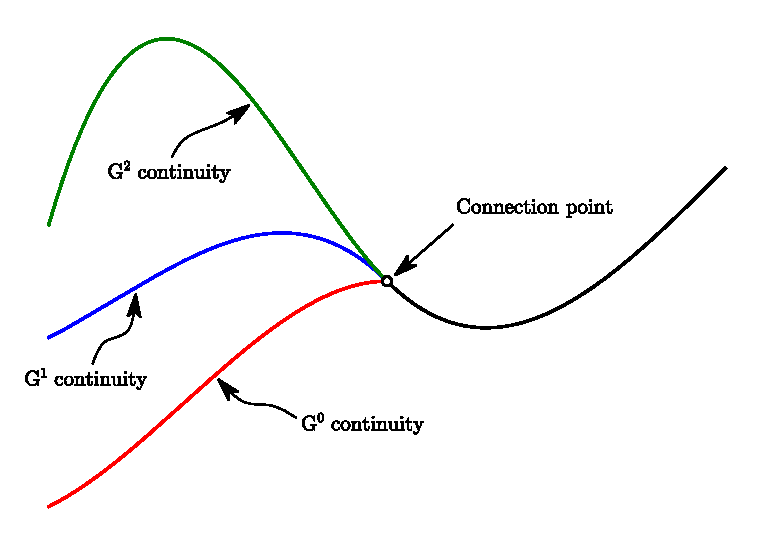
\includegraphics[width=0.8\linewidth]{1figures/curve_smoothness_annotated.pdf}
    \caption{Geometric continuity at the connection point between two curve segments}
    \label{fig:curve_smoothness}
\end{figure}

\begin{figure}[p]
    \centering
    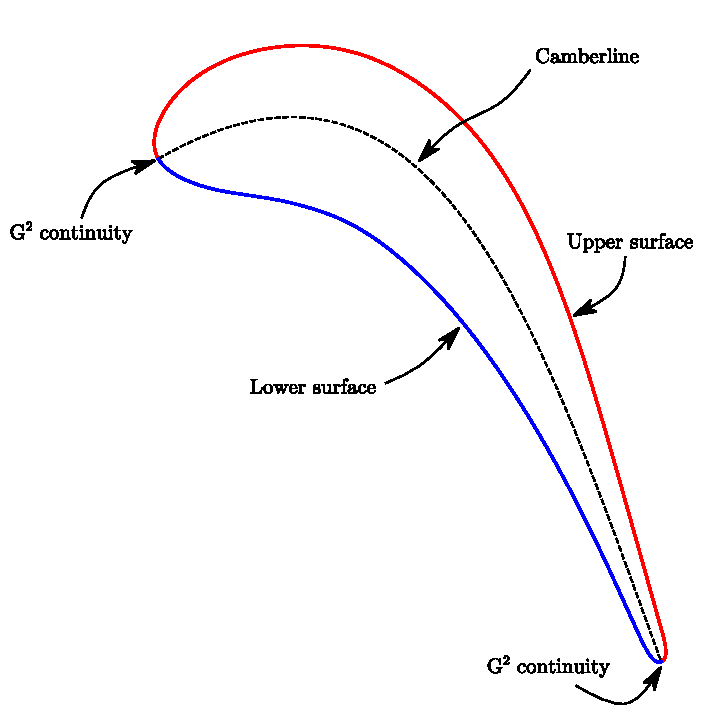
\includegraphics[width=0.8\linewidth]{1figures/G2_continutity_blade_annotated.pdf}
    \caption{G$^2$ continuity at the points connecting the upper and lower surfaces of and airfoil}
    \label{fig:G2_continutity_blade}
\end{figure}

\begin{figure}[p]
    \centering
    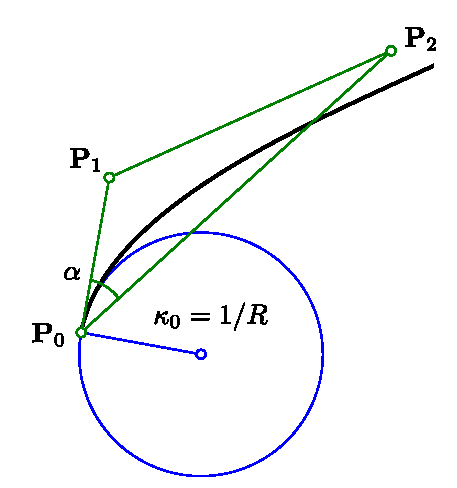
\includegraphics[width=0.5\linewidth]{1figures/endpoint_curvature_annotated.pdf}
    \caption{Curvature of a \Bezier or B-Spline curve at the endpoint $u=0$}
    \label{fig:endpoint_curvature}
\end{figure}

\begin{figure}[p]
    \centering
    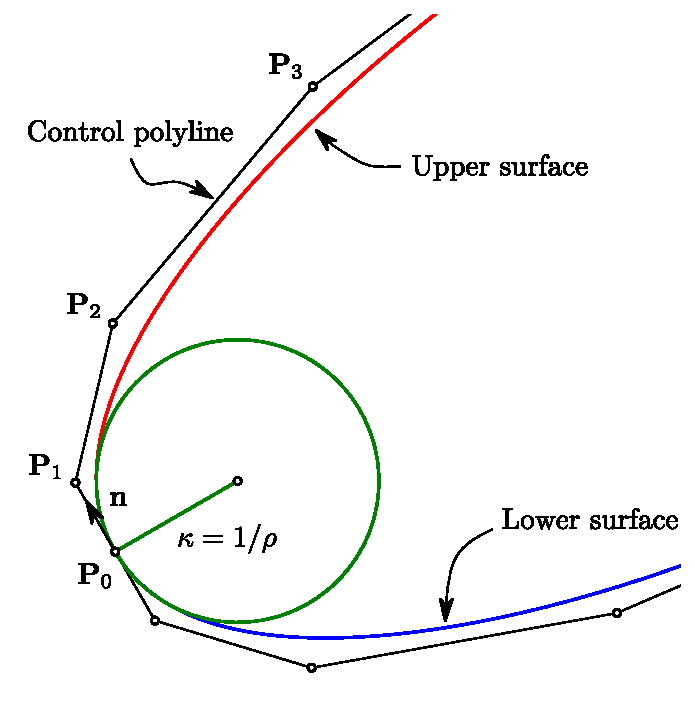
\includegraphics[width=0.65\linewidth]{1figures/leading_edge_construction_annotated.pdf}
    \caption{Construction of the leading edge of an airfoil ensuring G$^2$ continuity}
    \label{fig:leading_edge_construction}
\end{figure}





\end{document}